\documentclass[12pt]{article}
\usepackage{float}
\usepackage[table,xcdraw]{xcolor}
\usepackage{tikzit}
\input{Homework.tikzstyles}
\usepackage{hyperref}
\usepackage{amsmath}
\usepackage{amsfonts}
\usepackage{amssymb}
\usepackage{amsthm}
\usepackage{graphics}
\usepackage{graphicx}
\usepackage{yfonts}
\usepackage{float}
\usepackage[textwidth=16cm, textheight=22cm]{geometry}
\usepackage{dsfont}
\usepackage[nottoc]{tocbibind}
\setcounter{tocdepth}{3}
\setcounter{secnumdepth}{3}
\usepackage{url}
\usetikzlibrary{positioning}
\usepackage{neuralnetwork} 
\usepackage{multirow}
\usepackage{subcaption}
\usepackage{caption}
\usepackage[font=scriptsize]{caption}
\usepackage{ctable}
\usepackage{caption}
\usepackage{pifont}
\usepackage{array}
\usepackage{multirow}
\usepackage{subcaption}
\usepackage{ctable}
\usepackage{adjustbox}
\usepackage{booktabs}
\usepackage{tabularx, booktabs, makecell, caption}
\usepackage{siunitx}
\usepackage{booktabs}

\title{\textbf{\huge Investigating Intra-Layer Neuronal Mechanisms}\\[1ex]  \\[1ex] \\[1ex]}
\author{\Large{ Mohammad Zamani}  \\ \Large{Student No. 610399135} \\ \\ \Large{University of Tehran- CS Department}}
\date{}

\usepackage{titling}
\renewcommand\maketitlehooka{\null\mbox{}\vfill}
\renewcommand\maketitlehookd{\vfill\null}

\begin{document}
	%%%%%%%%%%%%%%%%%%%%%       Title Page      %%%%%%%%%%%%%%%%%%%%%%		

	
	\begin{titlingpage}
	
	\begin{figure}
		\centering
		
\includegraphics[width=0.3\textwidth]{Figs/University_of_Tehran_logo.png}		

	\end{figure}		\maketitle
	
	\end{titlingpage}
		
	


	%%%%%%%%%%%%%%%%%%%%%       Page 1       %%%%%%%%%%%%%%%%%%%%%%

	\setlength{\parindent}{20pt}
	\tableofcontents
	
	\vspace{1\baselineskip}

	\pagebreak

	\section{Introduction}
	
	This project delves into the intricacies of intra-layer neuronal mechanisms and their profound effects on learning processes within spiking neural networks. Using the CoNeX framework, we systematically implement and evaluate several key mechanisms, including Lateral Inhibition, k-Winners-Take-All, and Homeostasis, to understand their roles in shaping network behavior. Our approach involves training spiking neural networks with the Spike-Timing-Dependent Plasticity (STDP) learning rule, allowing us to observe the nuanced interactions between neurons within a layer.

Through a series of controlled experiments, we assess how different configurations and parameters of these mechanisms influence learning process and network performance. Specifically, we analyze how variations in neuronal sensitivity and competitive interactions affect the extraction of salient features and the overall learning trajectory. By comparing networks with different intra-layer mechanisms, we aim to identify optimal strategies that enhance learning outcomes.

Our results provide valuable insights into the dynamics of neural interactions within a layer and their critical impact on learning processes.


	\section{Experimental Setup}
	
	\subsection{Network Architecture}
	
	\hfill
	
	\subsubsection{First Architecture}
	
	In our previous project, we discussed a spiking neural network composed of two layers: an input layer and an output layer. The input layer contains two groups of neurons, each group having four neurons with distinct input patterns. The output layer consists of a single group with two neurons. We employed a fully connected pattern, where each neuron in the input layer is connected to all neurons in the output layer, as illustrated in Figure \ref{fig:na1}.

	
\begin{figure}[H]
\centering
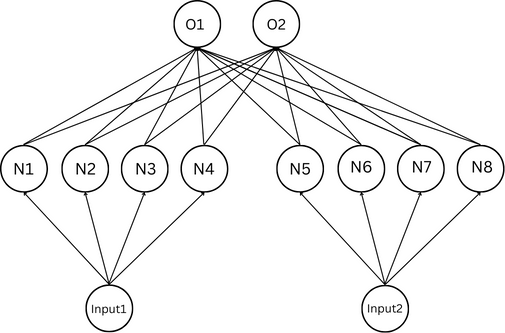
\includegraphics[width=0.45\textwidth]{Figs/inputq.png}
\caption{Network Architecture}
\label{fig:na1}
\end{figure}
\end{center}
	
	\subsubsection{Second Architecture} \label{SAN}
	
	
In this structure, we have a neuron group with five neurons in the output layer and five other neuron groups in the input layer, each consisting of four neurons. Each neuron in the input layer receives a distinct pattern as input. We used a full connectivity pattern, meaning every neuron in the input layer is connected to all five neurons in the output layer.

\begin{figure}[H]
\centering
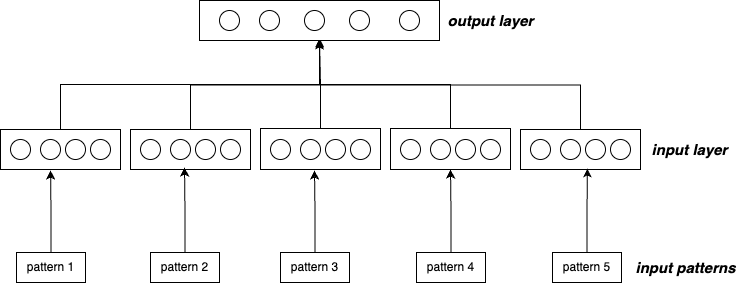
\includegraphics[width=0.85\textwidth]{Figs/nn.png}
\caption{Network Architecture}
\label{fig:na1}
\end{figure}
\end{center}


	
	\subsection{STDP Learning Rule}
	
	In the Spike-Timing-Dependent Plasticity (STDP) process, if an input spike to a neuron typically occurs just before the neuron’s output spike, the synaptic connection for that input is strengthened. Conversely, if an input spike generally occurs just after an output spike, the synaptic connection is weakened. This timing-dependent adjustment is the essence of "spike-timing-dependent plasticity." Consequently, inputs likely causing the post-synaptic neuron's excitation become more influential, while inputs that are unlikely to cause the excitation become less influential. Over time, this process refines the network by reinforcing a subset of connections while diminishing the impact of others to nearly zero. Since a neuron generates an output spike when many inputs arrive within a short time frame, the remaining subset of inputs tends to be those that are temporally correlated. Additionally, inputs that consistently precede the output spike and indicate early correlation become the primary inputs to the neuron, effectively optimizing the network for detecting and responding to relevant patterns.

	If we have two electrodes placed within the neuronal membrane, and we use one electrode to stimulate the neuron and the other to measure the neuron’s response, we can observe that if the previous neuron is activated and then the next connected neuron is activated shortly afterward, the synaptic strength between these two neurons increases. This indicates that the change in synaptic weight can be a function of the time difference  $ t_j^f - t_i^f $.
	
	
	

\begin{figure}[H]
\centering
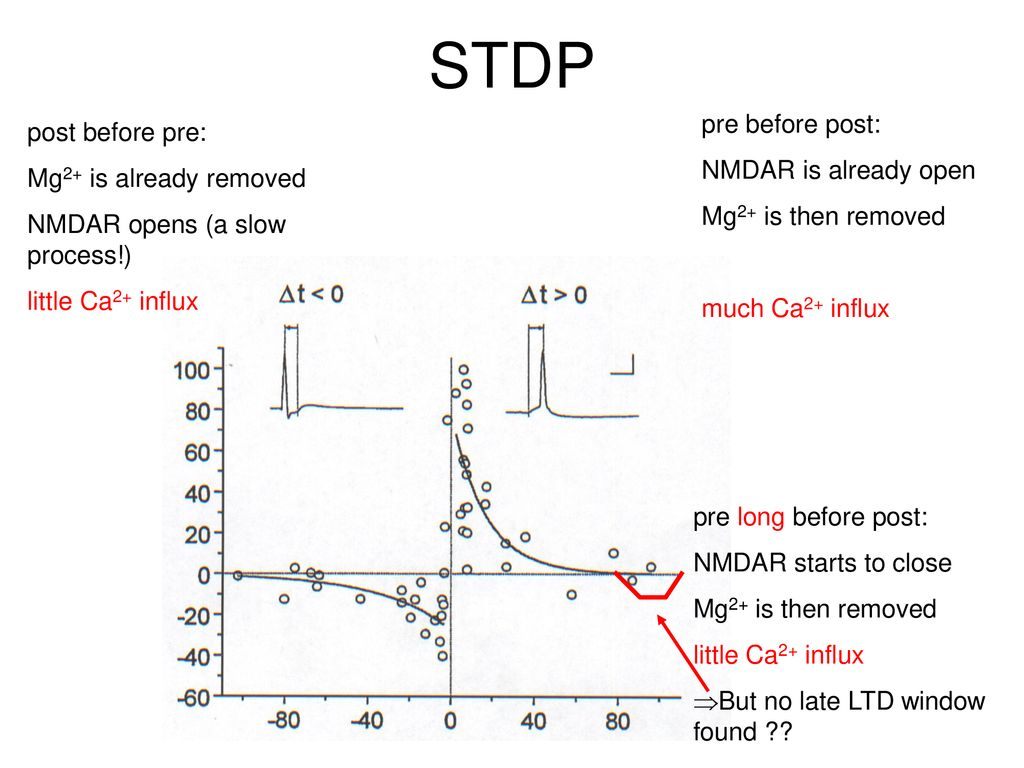
\includegraphics[width=10cm]{Figs/STDP.jpg}
\caption{STDP Leaning Process}
\label{Fig:p-d}
\end{figure}
\end{center}

LTP is the process by which synaptic strength is increased. It occurs when the presynaptic neuron fires just before the postsynaptic neuron. The closer in time these spikes occur, the stronger the synaptic connection becomes. The rationale behind LTP is that if a presynaptic neuron consistently helps to trigger a postsynaptic spike, it should be rewarded by strengthening the connection, making it easier to trigger future spikes. This process reinforces pathways that are frequently used, thereby promoting learning and memory formation.


LTD is the process by which synaptic strength is decreased. It occurs when the presynaptic neuron fires just after the postsynaptic neuron. The further apart these spikes occur, the weaker the synaptic connection becomes. LTD ensures that connections which do not contribute effectively to the postsynaptic activity are weakened. This pruning of less useful synapses is crucial for maintaining the efficiency of the neural network, preventing over-excitation, and ensuring that only the most relevant and effective synaptic pathways are strengthened.



In summary, the STDP learning process can be mathematically simulated using the following equation:

 $$ \frac{dw_{ij}}{dt} = -A_-(w_{ij})y_i(t)\Sigma_f \delta(t-t_j^f) + A_+(w_{ij})x_j(t)\Sigma_f \delta(t-t_i^f)$$
	
	\subsection{Parameter Configurations}
	
	\subsubsection{Input Patterns}
	
	For the input pattern, we used two images. These images were fed into a Poisson encoder, which then provided the encoded inputs to the neuron groups.
	
\begin{figure}[H]
\centering
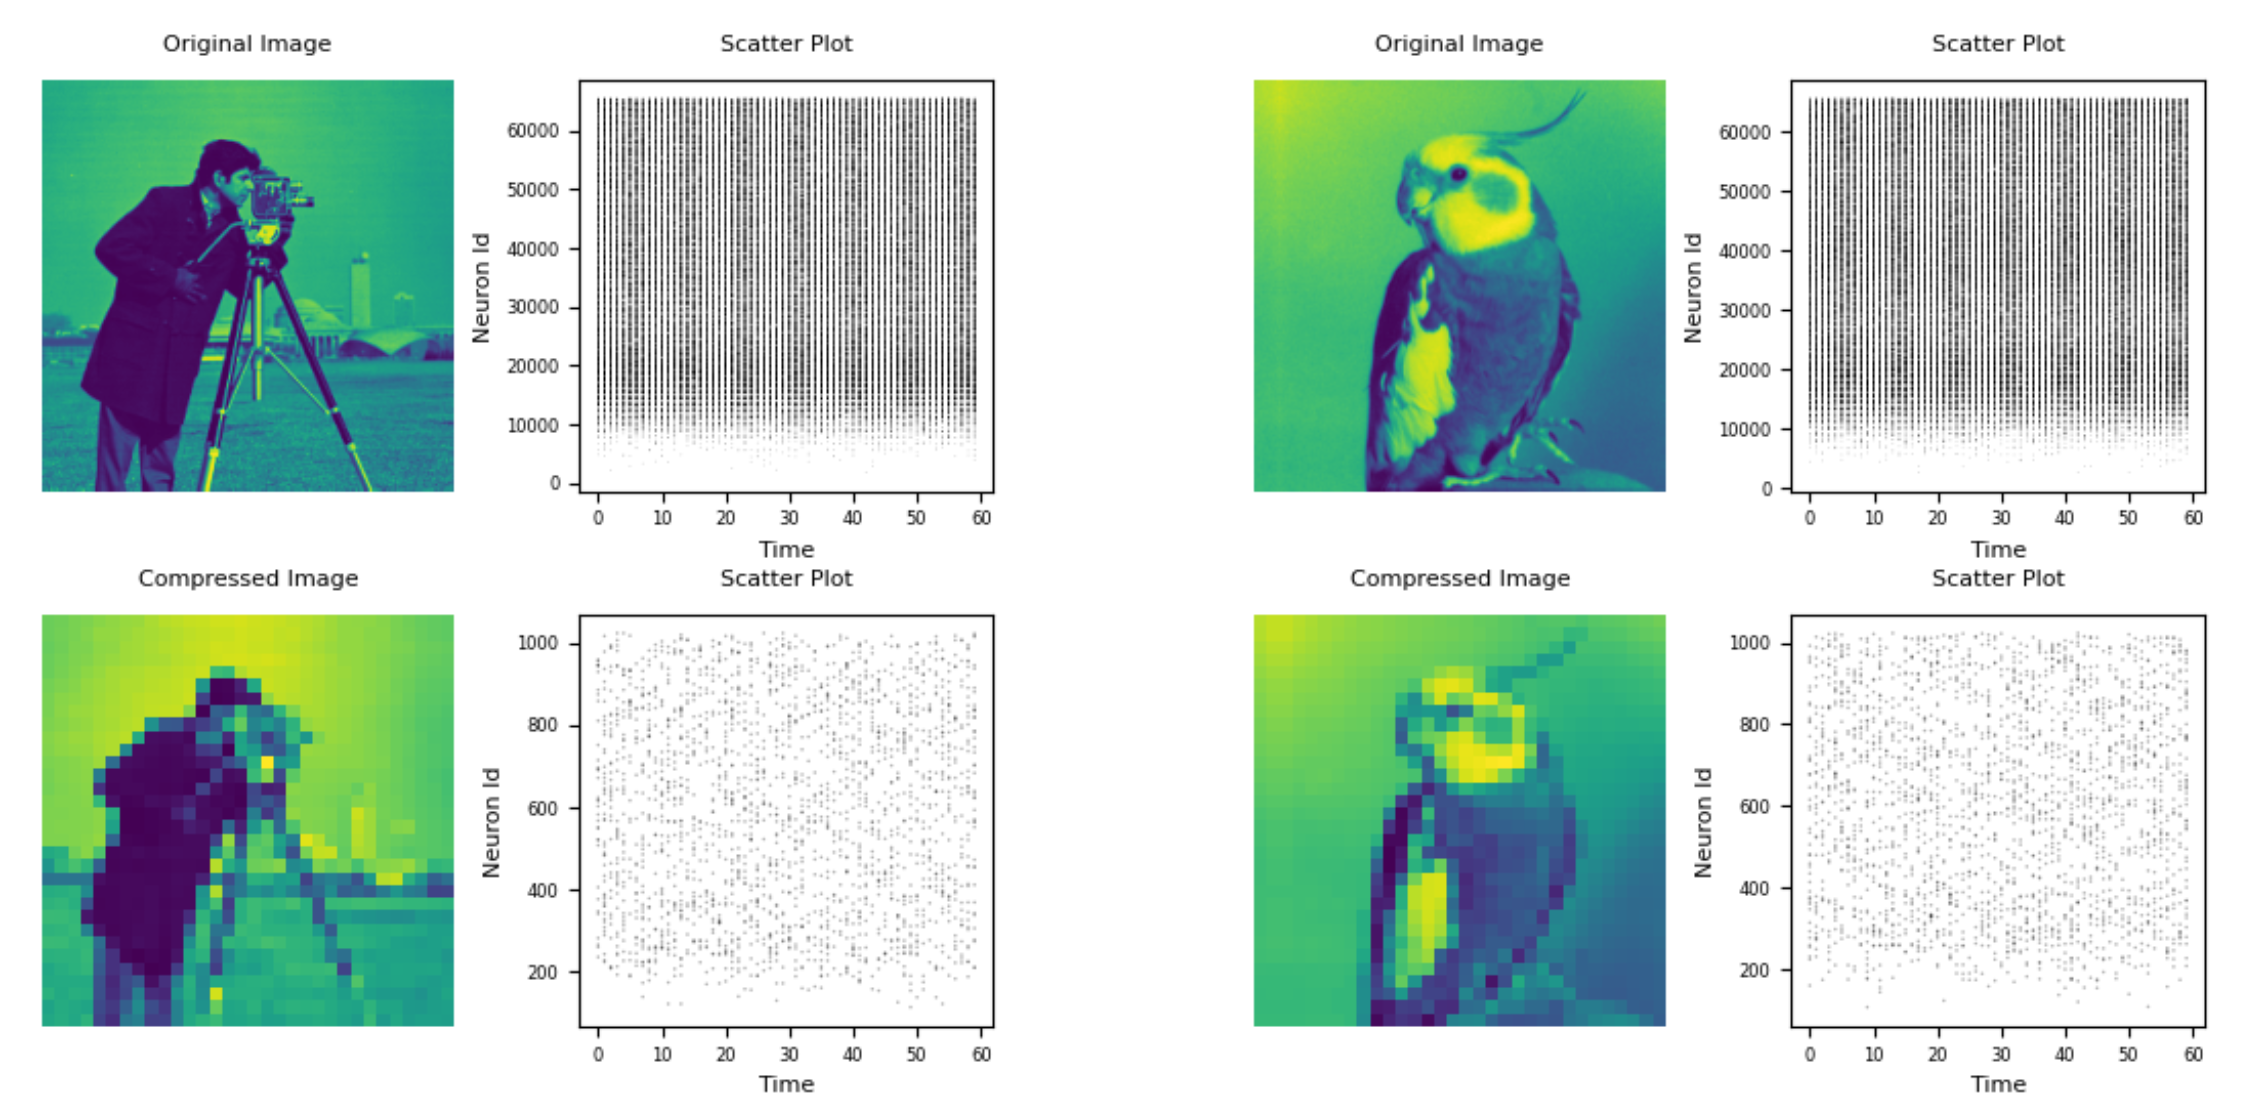
\includegraphics[width=13cm]{Figs/inputi}
\caption{Input images}
\label{Fig:inputimage}
\end{figure}
\end{center}

	\subsubsection{Spike Trace}
	
	The spike trace of each neuron is calculated by adding the current spike and decaying the existing trace. The key parameter in this calculation is the decay rate of the spike trace, which I have set to 1.
	
	\subsubsection{STDP Parameters}
	
	The most critical parameters in STDP learning are $A_+$ and  $A_-$, both of which I have set to 3. Additionally, I implemented a hard bound to control the weights.
	\subsubsection{Neuron Model}
	
	in the output layer we need to use a neuron model witch I used LIF neuron model with these parameters:
	$$  \tau=10, \;  U_{rest}=-65, \; U_{reset}=-70, \; threshold=-40, \; R=10 $$
	
	
	
	\section{Lateral Inhibition}
	
	Lateral inhibition is the phenomenon in which a neuron's response to a stimulus is inhibited by the excitation of a neighboring neuron. Lateral inhibition has been experimentally observed in the retina and the LGN of organisms. Lateral inhibition makes neurons more sensitive to spatially varying of stimulus than to spatially uniform stimulus. This is because a neuron getting stimulated by a spatially uniform stimulus is also inhibited by its surrounding neurons, thus suppressing its response. On the other hand, a neuron subjected to a spatially varying stimulus is less inhibited by its neighbors that are not excited, thus producing stronger response. Therefore in the case of visual neurons, lateral inhibition makes them more sensitive to edges on the scene. Although usually described for visual neurons, lateral inhibition is also found in other sensory systems, such as auditory and olfactory neurons. The total region, to which a particular neuron is sensitive to, is called the receptive field of the neuron.

The goal of this experiment is to determine if Lateral Inhibition can enhance the neural differentiation process, leading to a clearer and more distinct pattern recognition capability in the output neurons.


	\subsection{Different Input Pattern}
	
	For this experiment, we employed the first network structure with two distinct input patterns as detailed in the input patterns section. Figure \ref{fig} illustrates these patterns. Additionally, we incorporated a lateral inhibition mechanism in the output layer.

\begin{figure}[H]
\centering
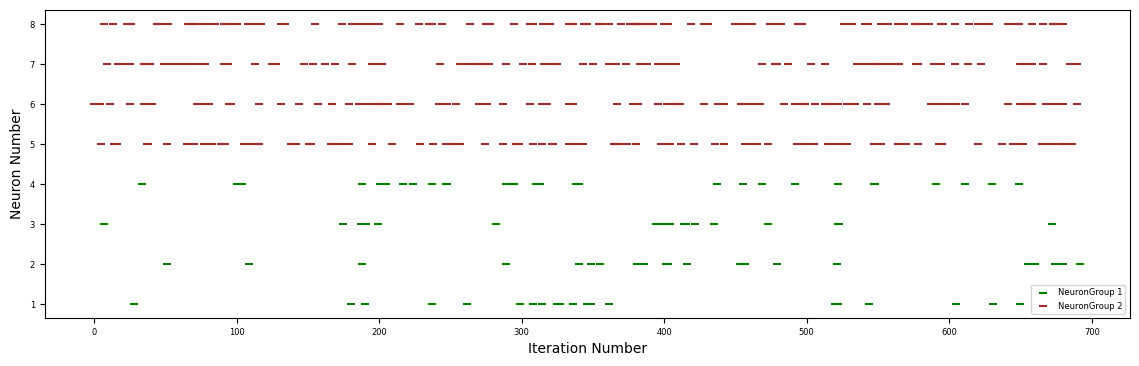
\includegraphics[width=15cm]{Figs/pattern.png}
\caption{Input Patterns}
\label{Fig:pattern}
\end{figure}
\end{center}

After 700 iterations of simulation, the resulting changes in weights are visible in Figure \ref{Fig:w-changes}. Subsequently, we calculated the cosine similarity between the weight vectors connected to the first and second output neurons. Specifically, each of the eight neurons in the input layer is connected to both the first and second output neurons, and we computed the cosine similarity of these weight vectors in every iteration.Figure \ref{fig:ce1} illustrates the evolution of cosine similarity during the simulation process.

\begin{figure}[H]
\centering
  \begin{subfigure}[b]{0.45\textwidth}
    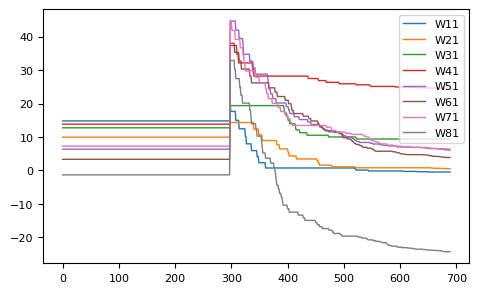
\includegraphics[width=\textwidth]{Figs/w1e1.png}
    \caption{Weights Connected to the First Output Neuron}
  \end{subfigure}
  \hspace*{10}
  \begin{subfigure}[b]{0.45\textwidth}
    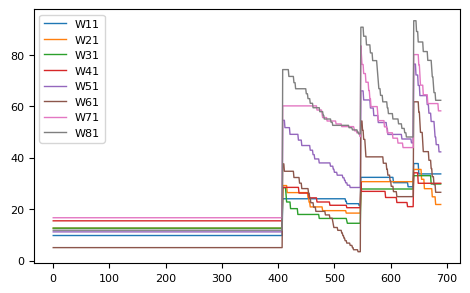
\includegraphics[width=\textwidth]{Figs/w2e1.png}
    \caption{Weights Connected to the Second Output Neuron}
  \end{subfigure}
  \caption{Weight Changes Throughout The Simulation}
  \label{Fig:w-changes}
\end{figure}
\end{center}


\begin{figure}[H]
\centering
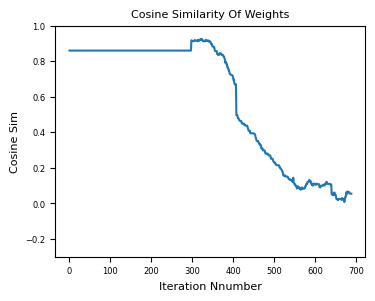
\includegraphics[width=0.40\textwidth]{Figs/ce1.png}
\caption{Cosine similarity during the simulation process}
\label{fig:ce1}
\end{figure}
\end{center}


If our task is classification, each output neuron represents a distinct class. The model performs effectively when the similarity between these output neurons is minimized, indicating clear differentiation among classes. Throughout the simulation, we observed a decrease in similarity between weights, illustrating the learning of distinct patterns by the output neurons. This outcome is desirable given our use of two distinct input patterns and the implementation of lateral inhibition in the output layer, which aimed to enhance differentiation. Consequently, the application of lateral inhibition increased the distinction between weights.

	\subsection{Different Input Pattern With Intersection}
	In this section, we provide the same input pattern to the first and second neurons of both neuron groups in the input layer. Thus, four out of the eight neurons in the input layer share the same pattern. The input patterns are illustrated in Figure \ref{Fig:pattern2}.
	
\begin{figure}[H]
\centering
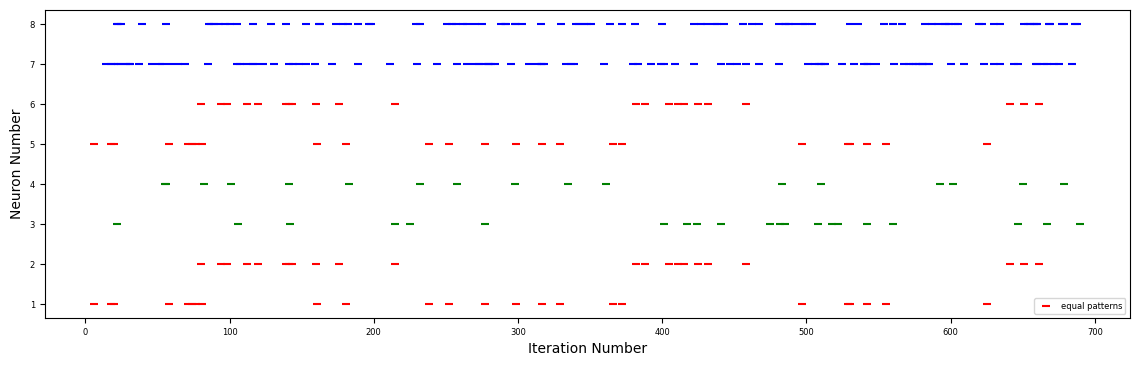
\includegraphics[width=15cm]{Figs/pattern2.png}
\caption{Input Patterns}
\label{Fig:pattern2}
\end{figure}
\end{center}



\begin{figure}[H]
\centering
  \begin{subfigure}[b]{0.45\textwidth}
    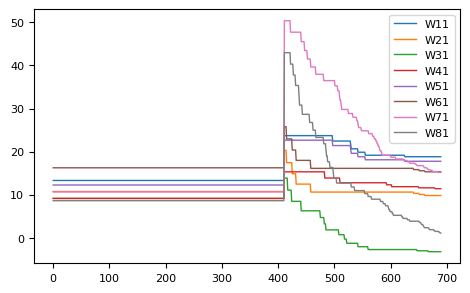
\includegraphics[width=\textwidth]{Figs/w1e2.png}
    \caption{Weights Connected to the First Output Neuron}
  \end{subfigure}
  \hspace*{10}
  \begin{subfigure}[b]{0.45\textwidth}
    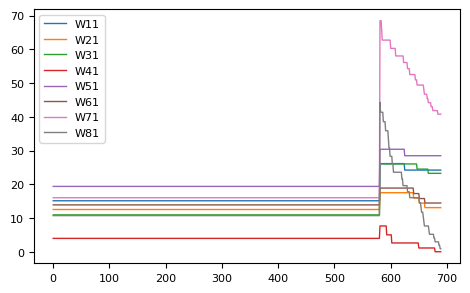
\includegraphics[width=\textwidth]{Figs/w2e2.png}
    \caption{Weights Connected to the Second Output Neuron}
  \end{subfigure}
  \caption{Weight Changes Throughout The Simulation}
  \label{Fig:w-changes2}
\end{figure}
\end{center}


As seen in Figure \ref{fig:ce2}, throughout the simulation, we observed a decrease in similarity between weights, illustrating the learning of distinct patterns by the output neurons. However, compared to Figure \ref{fig:ce1}, the decrease in weight similarity is much less. This indicates that increasing the overlap of input patterns makes differentiation harder. Nonetheless, with the use of lateral inhibition, there is still a small degree of distinction.

\begin{figure}[H]
\centering
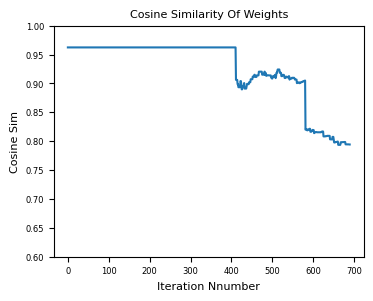
\includegraphics[width=0.40\textwidth]{Figs/ce2.png}
\caption{Cosine similarity during the simulation process}
\label{fig:ce2}
\end{figure}
\end{center}
	
	\subsection{Same Input Pattern} \label{SIP1}
	In this section, we provide the same input pattern to our input layer neurons. The input patterns are illustrated in Figure \ref{Fig:pattern2}.
	
	
	
As expected in this experiment, we provided identical input patterns to both input neuron groups. Initially, with weights following a normal distribution with a standard deviation of 10, the cosine similarity is approximately 1. After several simulation iterations, the cosine similarity remains around 1 because the input patterns are identical. Consequently, even lateral inhibition cannot differentiate between the patterns, which is expected behavior for our network. 


\begin{figure}[H]
\centering
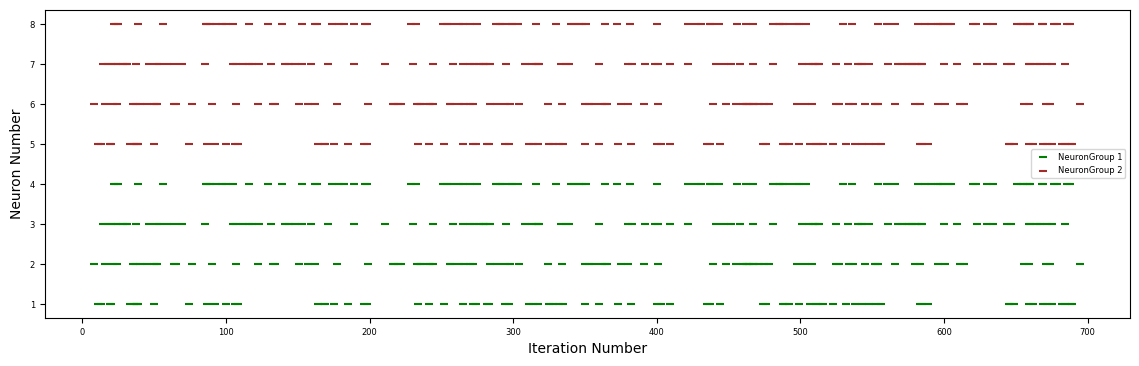
\includegraphics[width=15cm]{Figs/pattern3.png}
\caption{Input Patterns}
\label{Fig:pattern2}
\end{figure}
\end{center}



\begin{figure}[H]
\centering
  \begin{subfigure}[b]{0.45\textwidth}
    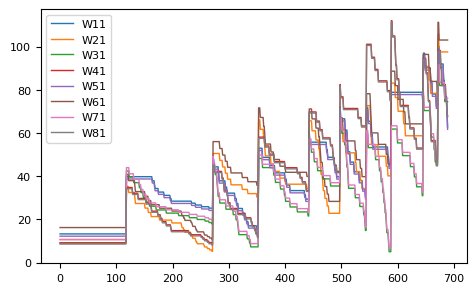
\includegraphics[width=\textwidth]{Figs/w1e3.png}
    \caption{Weights Connected to the First Output Neuron}
  \end{subfigure}
  \hspace*{10}
  \begin{subfigure}[b]{0.45\textwidth}
    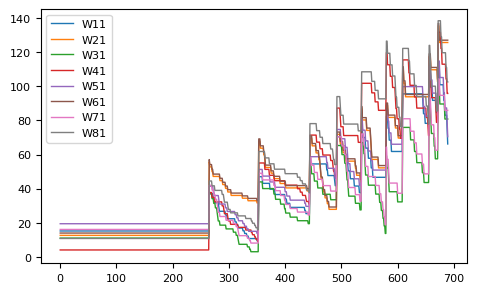
\includegraphics[width=\textwidth]{Figs/w2e3.png}
    \caption{Weights Connected to the Second Output Neuron}
  \end{subfigure}
  \caption{Weight Changes Throughout The Simulation}
  \label{Fig:w-changes3}
\end{figure}
\end{center}

\begin{figure}[H]
\centering
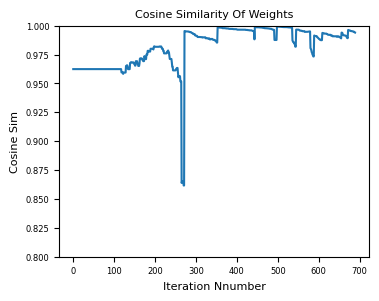
\includegraphics[width=0.40\textwidth]{Figs/ce3.png}
\caption{Cosine similarity during the simulation process}
\label{fig:ce2}
\end{figure}
\end{center}
		
		
	\section[KWTA]{KWTA\footnote{K Winners Take All}}
	
K-Winners-Take-All (KWTA) spiking neural networks are designed to select K elements from a total of N elements based on their activity levels, where the K selected elements have higher activation values than the remaining $N-K$ elements. When $𝐾=1$, the KWTA network functions as a Winner-Take-All (WTA) network, which identifies the neuron with the maximum activation.

Selecting the $K$ largest elements from a set of $N$ real numbers is crucial in decision-making, pattern recognition, associative memories, and competitive learning networks. Such tasks are common in classification problems and are essential for developing spiking neural network classifiers, as well as for solving pattern recognition and classification issues.

	
	The implementation concept of KWTA is that if  $ v \ge threshold$, then $v$ is set to $v_{reset}$, and all other spiked neurons are inhibited.
	
	\subsection{Different Input Pattern}
	
	
For this experiment, we used the first network structure with two distinct input patterns, as described in the input patterns section. Figure \ref{fig} illustrates these patterns. Additionally, we incorporated a lateral inhibition mechanism and k-Winners-Take-All (KWTA) in the output layer. Since we have two neurons in the output layer, we set $K = 1$. This setting allows us to distinguish between the two output neurons: the more active neuron inhibits the other, thereby differentiating between the patterns.

\begin{figure}[H]
\centering
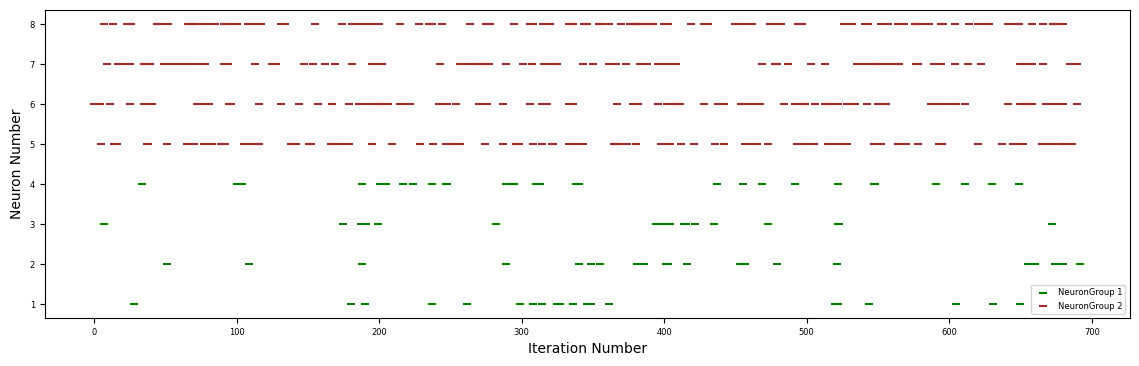
\includegraphics[width=15cm]{Figs/inputpattern.png}
\caption{Input Patterns}
\label{Fig:pattern5}
\end{figure}
\end{center}


As shown in Figure \ref{Fig:pattern5}, the second neuron group exhibits more activity throughout the simulation. Based on the KWTA algorithm, the second output neuron, representing the second neuron group pattern, will inhibit the first output neuron, which corresponds to the first neuron group pattern. Consequently, as depicted in Figure \ref{Fig:wch1}, the weights connected to the first output neuron decrease, while the weights connected to the second output neuron increase throughout the simulation.

\begin{figure}[H]
\centering
  \begin{subfigure}[b]{0.45\textwidth}
    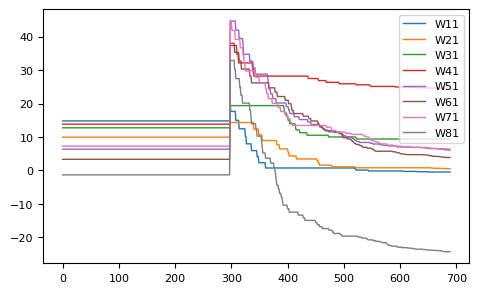
\includegraphics[width=\textwidth]{Figs/w1e4.png}
    \caption{Weights Connected to the First Output Neuron}
  \end{subfigure}
  \hspace*{10}
  \begin{subfigure}[b]{0.45\textwidth}
    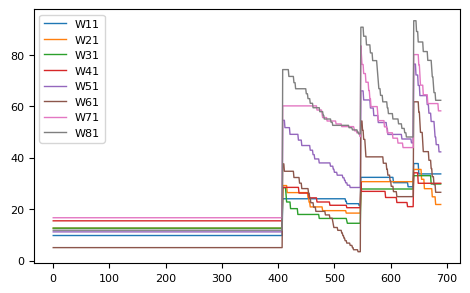
\includegraphics[width=\textwidth]{Figs/w2e4.png}
    \caption{Weights Connected to the Second Output Neuron}
  \end{subfigure}
  \caption{Weight Changes Throughout The Simulation}
  \label{Fig:wch1}
\end{figure}
\end{center}

Finally, Figure \ref{fig:ce4} shows the cosine similarity between weights throughout the simulation. By adding the KWTA mechanism with $k = 1$ in the output layer, the second output neuron inhibits the first output neuron more than before experiment. Although the effect of KWTA is not very obvious with only two neurons in the output layer, there is a notable decrease in cosine similarity between the weights compared to the before experiment, as shown in Figure \ref{fig:ce1} and Figure \ref{fig:ce4}. This indicates that the KWTA mechanism has helped to create a greater distinction between the patterns.

\begin{figure}[H]
\centering
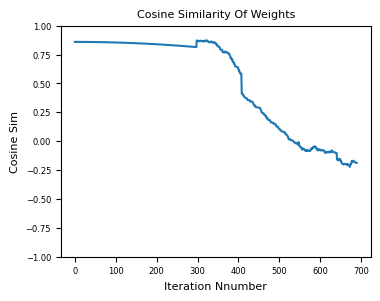
\includegraphics[width=0.40\textwidth]{Figs/ce4.png}
\caption{Cosine similarity during the simulation process}
\label{fig:ce4}
\end{figure}
\end{center}
	
	\subsection{Different Input Pattern With Intersection}
	
		In this section, we provide the same input pattern to the first and second neurons of both neuron groups in the input layer. Thus, four out of the eight neurons in the input layer share the same pattern. The input patterns are illustrated in Figure \ref{Fig:pattern6}.
		
\begin{figure}[H]
\centering
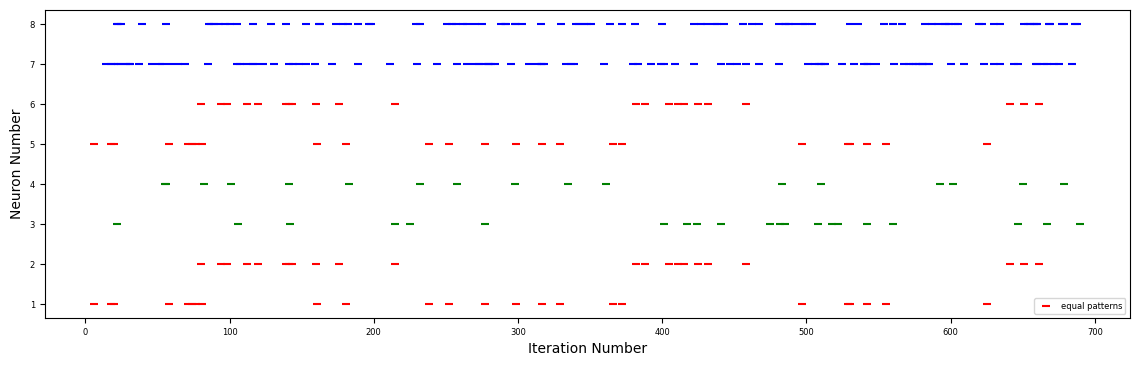
\includegraphics[width=15cm]{Figs/pattern6.png}
\caption{Input Patterns}
\label{Fig:patter62}
\end{figure}
\end{center}
	

For this experiment, as mentioned in the previous section, the second neuron group exhibits more activity, inhibiting the first output neuron. As a result, we observe a decrease in the weights connected to the first output neuron and an increase in the weights connected to the second output neuron throughout the simulation. This process is illustrated in Figure \ref{Fig:wch2}.
	
\begin{figure}[H]
\centering
  \begin{subfigure}[b]{0.45\textwidth}
    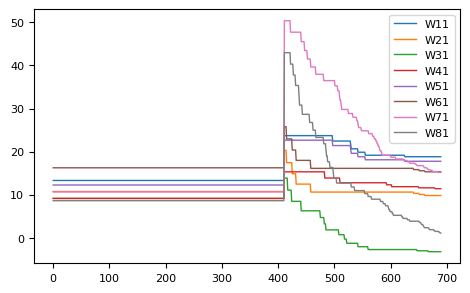
\includegraphics[width=\textwidth]{Figs/w1e5.png}
    \caption{Weights Connected to the First Output Neuron}
  \end{subfigure}
  \hspace*{10}
  \begin{subfigure}[b]{0.45\textwidth}
    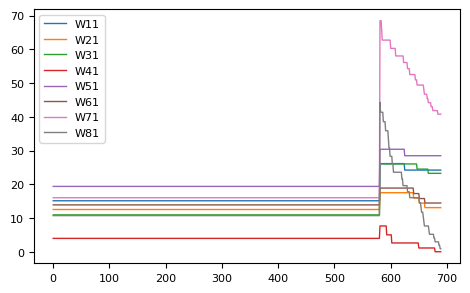
\includegraphics[width=\textwidth]{Figs/w2e5.png}
    \caption{Weights Connected to the Second Output Neuron}
  \end{subfigure}
  \caption{Weight Changes Throughout The Simulation}
  \label{Fig:wch2}
\end{figure}
\end{center}

\begin{figure}[H]
\centering
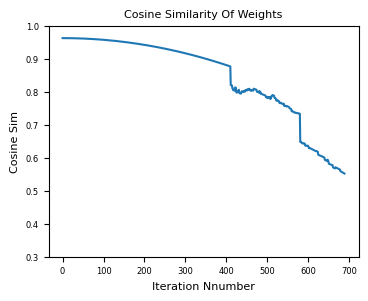
\includegraphics[width=0.40\textwidth]{Figs/ce5.png}
\caption{Cosine similarity during the simulation process}
\label{fig:ce5}
\end{figure}
\end{center}

In this section, since the patterns have intersections, there is less distinction between them, resulting in a smaller decrease in cosine similarity between weights. Figure \ref{fig:ce5} illustrates this phenomenon. However, when we used the KWTA mechanism in addition to the lateral inhibition mechanism, we achieved greater distinction between patterns. As shown in Figure \ref{Fig:c-c}, KWTA improved the classification of input patterns compared to using only the lateral inhibition mechanism.

\begin{figure}[H]
\centering
  \begin{subfigure}[b]{0.45\textwidth}
    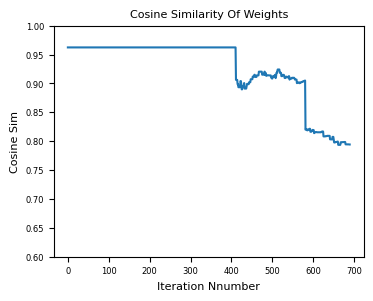
\includegraphics[width=\textwidth]{Figs/ce2.png}
    \caption{Used Only Lateral Inhibition In Output Layer}
  \end{subfigure}
  \hspace*{10}
  \begin{subfigure}[b]{0.45\textwidth}
    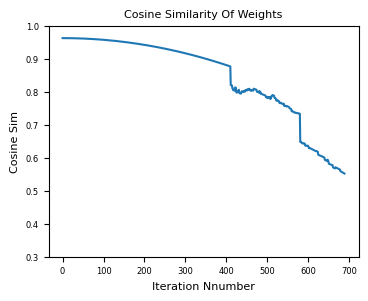
\includegraphics[width=\textwidth]{Figs/ce5.png}
    \caption{Used Lateral inhibition and KWTA In Output Layer}
  \end{subfigure}
  \caption{Cosine similarity during the simulation process}
  \label{Fig:c-c}
\end{figure}
\end{center}

		\subsection{Same Input Pattern}
		As I mentioned in \ref{SIP1}, when we have identical input patterns, it is evident that we cannot achieve any distinction. Even with the addition of KWTA, the behavior remains the same. There are minor weight changes due to the randomness of STDP, but throughout the simulation, the weights tend to become identical.
	
	
	\section{Homeostasis}

	\subsection{Homeostatic Process}
	
The human body consists of trillions of cells working together to maintain the organism's overall health and functionality. Despite their diverse functions, these cells share similar metabolic requirements. To ensure the well-being of both individual cells and the entire organism, it is crucial to maintain a constant internal environment that provides necessary elements such as oxygen, glucose, mineral ions, and waste removal. The various processes that regulate this internal environment are collectively known as homeostasis.

\subsection{Homeostasis}
Homeostasis refers to the stability, balance, or equilibrium of the body's internal environment. It involves the body's continuous efforts to maintain a constant and balanced state through persistent monitoring and adjustments in response to changing conditions. This process, known as homeostatic regulation, comprises three key components: the receptor, the control center, and the effector.

\begin{itemize}
\item The Receptor: Detects changes in the environment.
\item The Control Center: Receives and processes information from the receptor.
\item The Effector: Responds to the control center's commands by either opposing or enhancing the stimulus.
\end{itemize}

These components work together to restore and maintain homeostasis. For example, in regulating body temperature, temperature receptors in the skin send information to the brain (the control center), which then signals effectors such as blood vessels and sweat glands in the skin. Due to the constant changes in both the internal and external environment, the body must continuously make adjustments to stay at or near a specific value, known as the set point.

\begin{figure}[H]
\centering
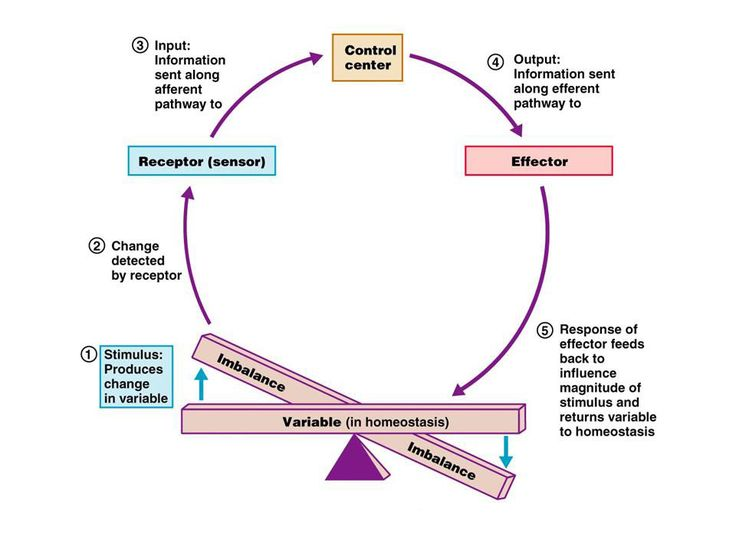
\includegraphics[width=0.7\textwidth]{Figs/h.jpg}
\caption{Homeostasis: positive/ negative feedback mechanisms example}
\label{fig:ce1}
\end{figure}
\end{center}


\subsection{Purpose of Homeostasis}

The primary goal of homeostasis is to maintain equilibrium around the set point. While there are normal fluctuations from this set point, the body's systems strive to return to it. When a stimulus causes a change in the internal or external environment, a receptor detects this change, and the system responds by adjusting the parameter back towards the set point. For instance, if the body becomes too warm, mechanisms are activated to cool it down. Similarly, if blood glucose levels rise after a meal, the body adjusts by moving glucose into tissues that need it or storing it for later use, thereby lowering the blood glucose level.

By continuously regulating these processes, homeostasis ensures the stability necessary for the cells and the organism to function optimally.


\subsection{Experiments}
In this experiment, we employed the second network architecture detailed in Section \ref{SAN}. For the input, we utilized five distinct patterns, each representing different images encoded using Poisson coding, as illustrated in Figure \ref{Fig:patter7}.



\begin{figure}[H]
\centering
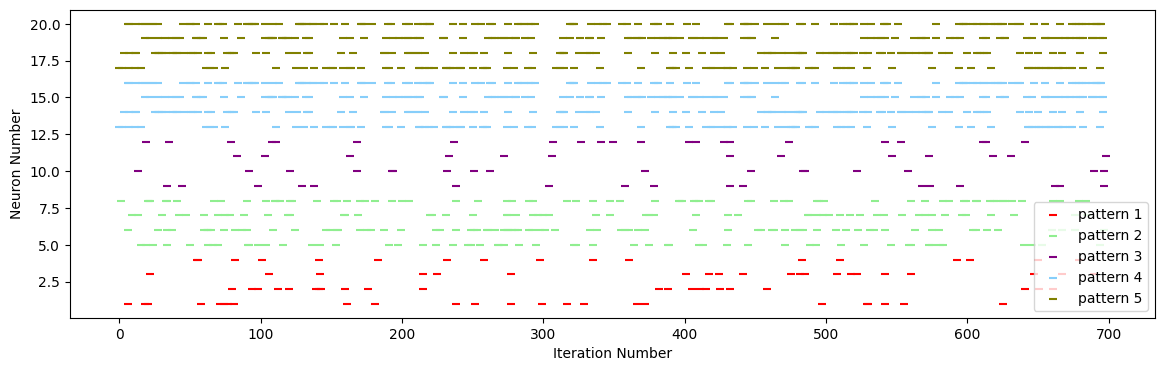
\includegraphics[width=16cm]{Figs/pattern7.png}
\caption{Input Patterns}
\label{Fig:patter7}
\end{figure}
\end{center}


In our experiment, we utilized five output neurons, with each neuron corresponding to one of the distinct input patterns. Additionally, 20 neurons from the input layer were connected to each of these output neurons, facilitating a complex network of interactions.

Figure \ref{Fig:w-w} illustrates the weight changes for a specific output neuron throughout the simulation process. Given the diversity of input patterns, the weight changes were not uniform across the neurons. However, some patterns exhibited similarities in their weight changes. For instance, the weight changes for the fourth and second neuron groups were quite similar, reflecting the likeness in their input patterns. A similar situation was observed for the first and third neuron groups, where the weight changes closely likely each other. These similarities indicate that input patterns with analogous features result in comparable weight adjustments during the learning process.


\begin{figure}[H]
\centering
  \begin{subfigure}[b]{0.45\textwidth}
    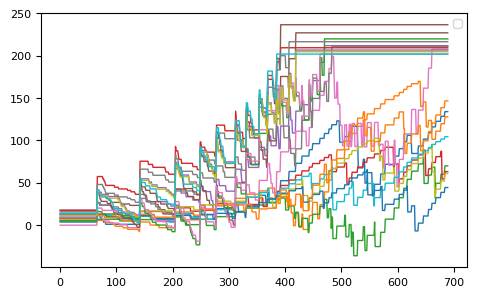
\includegraphics[width=\textwidth]{Figs/w1.png}
    \caption{Weights Connected to the First Output Neuron}
  \end{subfigure}
  \hspace*{10}
  \begin{subfigure}[b]{0.45\textwidth}
    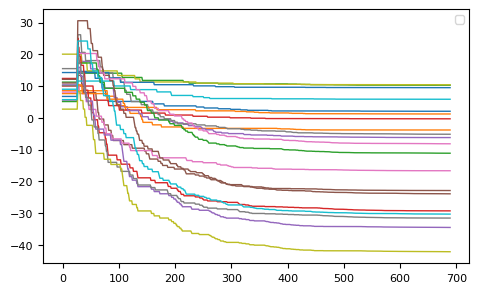
\includegraphics[width=\textwidth]{Figs/w2.png}
    \caption{Weights Connected to the Second Output Neuron}
  \end{subfigure}
  \\[\smallskipamount]
  \begin{subfigure}[b]{0.45\textwidth}
    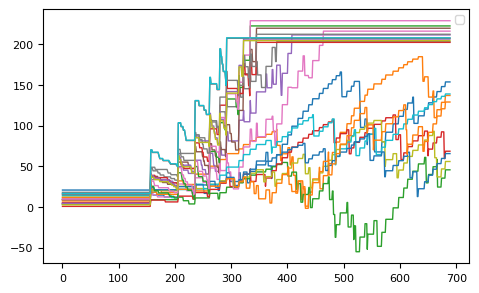
\includegraphics[width=\textwidth]{Figs/w3.png}
    \caption{Weights Connected to the Third Output Neuron}
  \end{subfigure}
  \hspace*{10}
  \begin{subfigure}[b]{0.45\textwidth}
    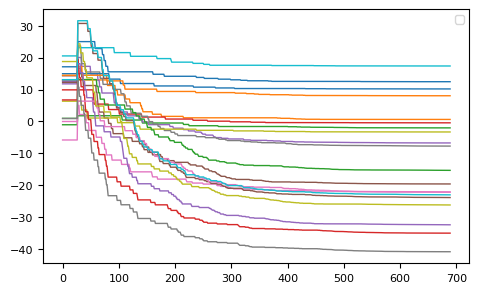
\includegraphics[width=\textwidth]{Figs/w4.png}
    \caption{Weights Connected to the Fourth Output Neuron}
  \end{subfigure}
  \\[\smallskipamount]
  \begin{subfigure}[b]{0.45\textwidth}
    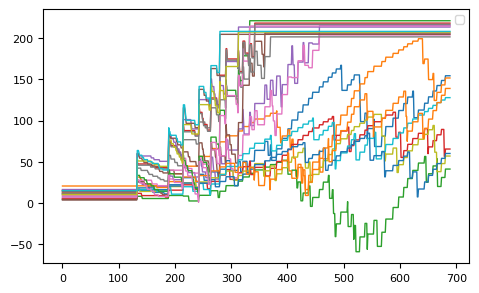
\includegraphics[width=\textwidth]{Figs/w5.png}
    \caption{Weights Connected to the Fifth Output Neuron}
  \end{subfigure}
  \caption{Weight Changes Throughout The Simulation}
  \label{Fig:w-w}
\end{figure}
\end{center}

Finally, for each combination of weights, we defined the cosine similarity of the weights throughout the simulation process. We have 10 different combinations. Figure \ref{Fig:c:c} shows the results of the cosine similarities.


\subsection{Conclusion}

One of the challenges we encounter in classifying these patterns is the variable distribution of spike counts within the input data. For instance, some activity classes, like the second input pattern, exhibit a large number of active neurons, whereas other classes, like the third input pattern, involve only a few active neurons. This discrepancy in distribution across different classes can introduce a bias in the learning process, favoring high-activity classes because the neurons corresponding to these classes become the winners. Moreover, the learning progress for classes with lower neuron activity typically proceeds at a slower pace. To mitigate this issue, we employed a decision homeostasis mechanism aimed at addressing these challenges.


\begin{figure}[H]
\centering
  \begin{subfigure}[b]{0.30\textwidth}
    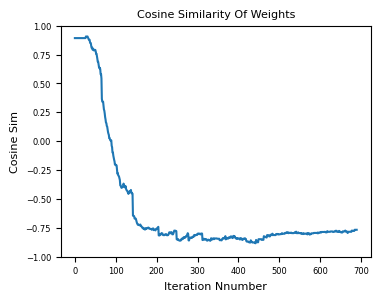
\includegraphics[width=\textwidth]{Figs/0-1.png}
    \caption{first and second}
  \end{subfigure}
  \hspace*{10}
  \begin{subfigure}[b]{0.3\textwidth}
    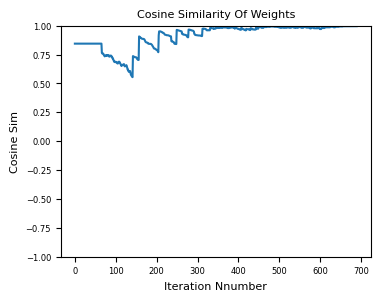
\includegraphics[width=\textwidth]{Figs/0-2.png}
    \caption{first and third}
  \end{subfigure}
  \hspace*{10}
  \begin{subfigure}[b]{0.3\textwidth}
    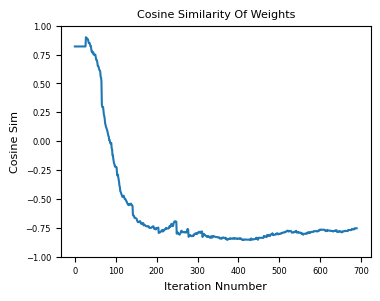
\includegraphics[width=\textwidth]{Figs/0-3.png}
    \caption{first and fourth}
  \end{subfigure}
  \\[\smallskipamount]
  \begin{subfigure}[b]{0.3\textwidth}
    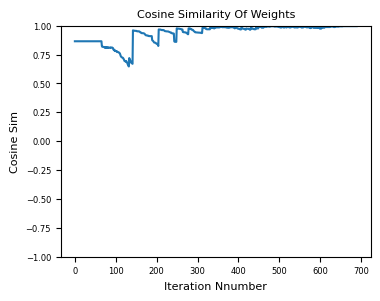
\includegraphics[width=\textwidth]{Figs/0-4.png}
    \caption{first and fifth}
  \end{subfigure}
  \hspace*{10}
  \begin{subfigure}[b]{0.3\textwidth}
    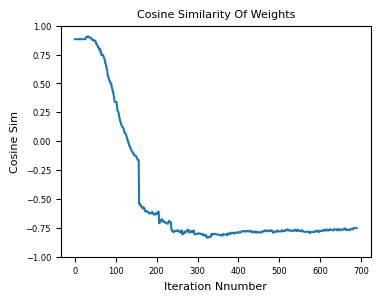
\includegraphics[width=\textwidth]{Figs/1-2.png}
    \caption{second and third}
  \end{subfigure}
  \hspace*{10}
  \begin{subfigure}[b]{0.3\textwidth}
    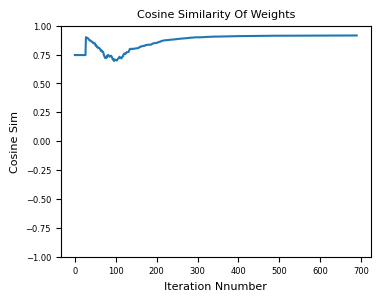
\includegraphics[width=\textwidth]{Figs/1-3.png}
    \caption{second and fourth}
  \end{subfigure}
  \\[\smallskipamount]
 
  \begin{subfigure}[b]{0.3\textwidth}
    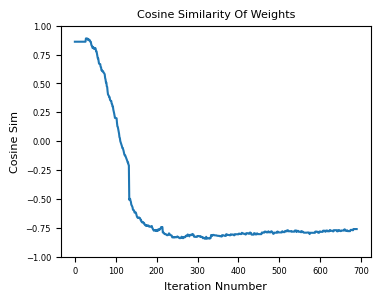
\includegraphics[width=\textwidth]{Figs/1-4.png}
    \caption{second and fifth}
  \end{subfigure}
  \hspace*{10}
  \begin{subfigure}[b]{0.3\textwidth}
    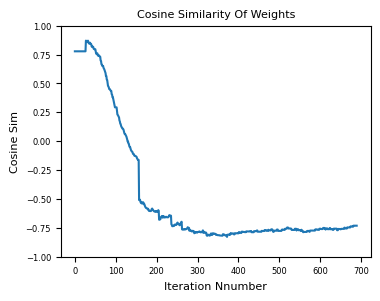
\includegraphics[width=\textwidth]{Figs/2-3.png}
    \caption{third and fourth}
  \end{subfigure}
  \hspace*{10}
  \begin{subfigure}[b]{0.3\textwidth}
    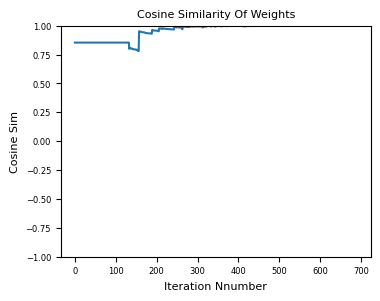
\includegraphics[width=\textwidth]{Figs/2-4.png}
    \caption{third and fifth}
  \end{subfigure}
   \\[\smallskipamount]
  \begin{subfigure}[b]{0.3\textwidth}
    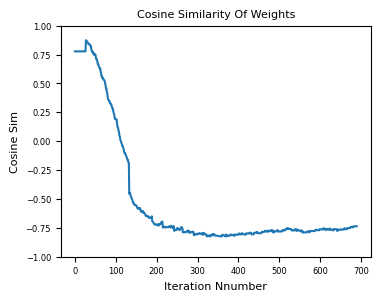
\includegraphics[width=\textwidth]{Figs/3-4.png}
    \caption{fourth and fifth}
  \end{subfigure}
  \caption{Cosine similarity between the input weights of two output neurons during the simulation process}
  \label{Fig:c:c}
\end{figure}


\end{center}



	
\end{document}